\newcommand\name{\subsecname: Construction Example}
\begin{frame}{\name}
$L1:L5:R2\enspace\xmapsto{\overset\Longleftarrow{R5}(\overline{Lp})}\enspace???$

\begin{itemize}
    \item Identify $Lp$\\
    $$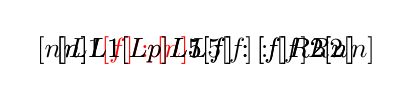
\begin{tikzpicture}
        \node<+> at(0,0){$[n]L1{\color{red}[f]:[n]}L5[f]:[f]R2[n]$};
        \node<+> at(0,0){$[n]L1{\color{red}[Lp]}L5[f]:[f]R2[n]$};
        \node<+-> at(0,0){$[n]L1[Lp]L5[f]:[f]R2[n]$};
    \end{tikzpicture}$$
    \item<+-> Only the segment between $L5$ and $R2$ is intermediate
    $$
      \underline{R2n=L1n}<L1<{\color{red}Lp}=L5n<\underline{L5f=R2f}<{\color{red}R5}
      $$
    
\end{itemize}
\end{frame}

\begin{frame}{\name}
$L1:L5:R2\enspace\xmapsto{\overset\Longleftarrow{R5}(\overline{Lp})}\enspace???$\\
\vfill
Found $L5f=R2f$ as an intermediate segment
\begin{itemize}
    \item<1-> Insert crossings $x_1$ and $x_2$ at intermediate segment
    \note<3>[item]{under because our finger is going above}
    $$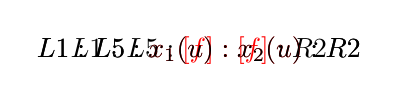
\begin{tikzpicture}
        \node<2> at(0,0){$L1:L5:{\color{red}[f]:[f]}:R2$};
        \node<3> at(0,0){$L1:L5:{\color{red}x_1(u):x_2(u)}:R2$};
        \node<4-> at(0,0){$L1:L5:x_1(u):x_2(u):R2$};
    \end{tikzpicture}$$
    \item<4-> Insert $R5$ at $Lp$ with $x_1$ and $x_2$
    $$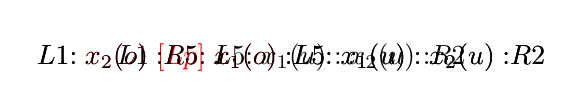
\begin{tikzpicture}
        \node<5> at(0,0){$\stackrel\curvearrowright{L1}{\color{red}[Lp]}\stackrel\curvearrowright{L5}:x_1(u):x_2(u):\stackrel\curvearrowright{R2}$};
        \node<6> at(0,0){$\stackrel\curvearrowright{L1}:{\color{red}x_2(o):\stackrel\curvearrowleft{R5}:x_1(o)}:\stackrel\curvearrowright{L5}:x_1(u):x_2(u):\stackrel\curvearrowright{R2}$};
        \node<7-> at(0,0){$\stackrel\curvearrowright{L1}:x_2(o):\stackrel\curvearrowleft{R5}:x_1(o):\stackrel\curvearrowright{L5}:x_1(u):x_2(u):\stackrel\curvearrowright{R2}$};
    \end{tikzpicture}$$
    $$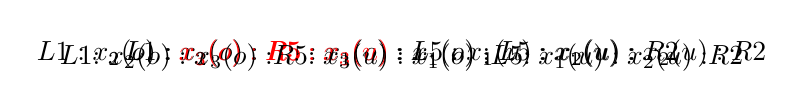
\begin{tikzpicture}
        \node<8> at(0,0){$L1:x_2(o):{\color{red}R5}:x_1(o):L5:x_1(u):x_2(u):R2$};
        \node<9> at(0,0){$L1:x_2(o):{\color{red}x_3(o):R5:x_3(u)}:x_1(o):L5:x_1(u):x_2(u):R2$};
        \node<10-> at(0,0){$\stackrel\curvearrowright{L1}:x_2(o):{x_3(o):\stackrel\curvearrowright{R5}:x_3(u)}:x_1(o):\stackrel\curvearrowright{L5}:x_1(u):x_2(u):\stackrel\curvearrowright{R2}$};
    \end{tikzpicture}$$
\end{itemize}
\end{frame}
\note[itemize]{
\item and this is our final result, lets check with the diagram
}

\begin{frame}{\name}
$$\scriptstyle
L1:L5:R2\enspace\xmapsto{\overset\Longleftarrow{R5}(\overline{Lp})}\enspace\stackrel\curvearrowright{L1}:x_2(o):{x_3(o):\stackrel\curvearrowright{R5}:x_3(u)}:x_1(o):\stackrel\curvearrowright{L5}:x_1(u):x_2(u):\stackrel\curvearrowright{R2}
$$

\begin{center}
\g[0.4]{figures/star-before}$\xmapsto{\overset\Longleftarrow{R5}(\overline{Lp})}$
\g[0.4]{figures/star-pick-twist}
\end{center}
\end{frame}
